%% Template basiert auf der Vorlage der Uni Graz für VWA: https://latex.tugraz.at/vorlagen/allgemein

%% Versionen:
%% V1: 9. Augugst 2021 (GreiA)



%% %%%%%%%%%%%%%%%%%%%%%%%%%%%%%%%%%%%%%%%%%%%%%%%%%%%%%%%%%%%%%%%%%%%
%% Allgemeine Festlegungen für die Darstellung des Gesamtdokumentes;
%% %%%%%%%%%%%%%%%%%%%%%%%%%%%%%%%%%%%%%%%%%%%%%%%%%%%%%%%%%%%%%%%%%%%
\newcommand{\mypapersize}{A4}
%% e.g., "A4", "letter", "legal", "executive", ...
%% The size of the paper of the resulting PDF file.

\newcommand{\mylaterality}{twoside}
%% "oneside" or "twoside"
%% Either you are creating a document which is printed on both, left pages
%% and right pages (twoside) or you create a document which is printed
%% on right pages only (oneside).

\newcommand{\mydraft}{false}
%% "true" or "false"
%% Use draft mode? If true, included graphics are replaced by empty
%% rectangles (of same size) and overfull boxes (in margin space) are
%% marked with black box (-> easy to spot!)

\newcommand{\myparskip}{half}
%% e.g., "no", "full", "half", ...
%% How to separate paragraphs: indention ("no") or spacing ("half",
%% "full", ...).

\newcommand{\myBCOR}{0mm}
%% Inner binding correction. This value depends on the method which is
%% being used to bind your printed result. Some techniques do not
%% require a binding correction at all ("0mm"), other require for
%% example "5mm". Refer to KOMA script documentation for a detailed
%% explanation what a binding correction is and how to measure it.

\newcommand{\myfontsize}{12pt}
%% e.g., 10pt, 11pt, 12pt
%% The font size of the main text in pt (points).

\newcommand{\mylinespread}{1.0}
%% e.g., 1.0, 1.5, 2.0
%% Line spacing in %/100. For example 1.5 means 150% of the usual line
%% spacing. Please use with caution: 100% ("1.0") is fine because the
%% font was designed for it.

\newcommand{\mylanguage}{ngerman, american}
%% "english,ngerman", "ngerman,english", ...
%% NOTE: The *last* language is the active one!
%% See babel documentation for further details.

%% BibLaTeX-settings: (see biblatex reference for further description)
\newcommand{\mybiblatexstyle}{authoryear}
%% e.g., "alphabetic", "authoryear", ...
%% The biblatex style which is being used for referencing. See
%% biblatex documentation for further details and more values.
%%
%% CAUTION: if you change the style, please check for (in)compatible
%%          "biblatex" package options in the file
%%          "template/preamble.tex"! For example: "alphabetic" does
%%          not have an option "dashed=..." and causes an error if it
%%          does not get removed from the list of options.

\newcommand{\mybiblatexdashed}{false}  %% "true" or "false"
%% If true: replace recurring reference authors with a dash.

\newcommand{\mybiblatexbackref}{true}  %% "true" or "false"
%% If true: create backward links from reference to citations.

\newcommand{\mybiblatexfile}{references-biblatex.bib}
%% Name of the biblatex file that holds the references.

\newcommand{\mydispositioncolor}{30,103,182}
%% e.g., "30,103,182" (blue/turquois), "0,0,0" (black), ...
%% Color of the headings and so forth in RGB (red,green,blue) values.
%% NOTE: if you are using "0,0,0" for black, printers might still
%%       recognize pages as color pages. In case this is a problem
%%       (paying for color print-outs vs. paying for b/w-printouts)
%%       please edit file "template/preamble.tex" and change
%%       "\definecolor{DispositionColor}{RGB}{\mydispositioncolor}"
%%       to "\definecolor{DispositionColor}{gray}{0}" and thus
%%       overwriting the value of \mydispositioncolor above.

\newcommand{\mycolorlinks}{true}  %% "true" or "false"
%% Enables or disables colored links (hyperref package).



\newcommand{\mytitlepage}{template/title_thesis_htlinn} %Titelseite

\newcommand{\mytodonotesoptions}{}
%% e.g., "" (empty), "disable", ...
%% Options for the todonotes-package. If "disable", all todonotes will
%% be hidden (including listoftodos).

%% Load main settings for document preamble:
\documentclass[%
fontsize=\myfontsize,%% size of the main text
paper=\mypapersize,  %% paper format
parskip=\myparskip,  %% vertical space between paragraphs (instead of indenting first par-line)
DIV=calc,            %% calculates a good DIV value for type area; 66 characters/line is great
headinclude=true,    %% is header part of margin space or part of page content?
footinclude=false,   %% is footer part of margin space or part of page content?
open=right,          %% "right" or "left": start new chapter on right or left page
appendixprefix=true, %% adds appendix prefix; only for book-classes with \backmatter
bibliography=totoc,  %% adds the bibliography to table of contents (without number)
draft=\mydraft,      %% if true: included graphics are omitted and black boxes
                     %%          mark overfull boxes in margin space
BCOR=\myBCOR,        %% binding correction (depends on how you bind
                     %% the resulting printout.
\mylaterality        %% oneside: document is not printed on left and right sides, only right side
                     %% twoside: document is printed on left and right sides
]{scrbook}  %% article class of KOMA: "scrartcl", "scrreprt", or "scrbook".
            %% CAUTION: If documentclass will be changed, *many* other things
            %%          change as well like heading structure, ...

\usepackage{float}
\usepackage{ifthen}
\usepackage[T1]{fontenc}
\usepackage{lmodern}
\usepackage[utf8]{inputenc} %% UTF8 as input characters
\usepackage{textcomp}
\usepackage[\mylanguage]{babel}  %% used languages; default language is *last* language of options
\usepackage{scrlayer-scrpage} %%  advanced page style using KOMA


\ifthenelse{\boolean{\mydraft}}{   %% the \mydraft switches between
                                   %% showing rectangles instead of graphics
  \usepackage[pdftex,draft]{graphicx}
}
{
  \usepackage[pdftex]{graphicx}
}

\usepackage{pifont}
%% pre-define ifthen-boolean variables:
\newboolean{myaddcolophon}
\newboolean{myaddlistoftodos}
\newboolean{english_affidavit}
\usepackage{xspace}
\usepackage[usenames,dvipsnames]{xcolor}
\definecolor{DispositionColor}{RGB}{\mydispositioncolor} %% used for links and so forth in screen-version

\usepackage[normalem]{ulem}
\usepackage{framed}
\usepackage{eso-pic}
\usepackage{enumitem}
\usepackage[\mytodonotesoptions]{todonotes}  %% option "disable" removes all todonotes output from 
\usepackage{units}
\usepackage{listings}
%% DO NOT REMOVE THIS LINE!

\setboolean{myaddcolophon}{true}  %% "true" or "false"
%% If set to "true": a colophon (with notes about this document
%% template, LaTeX, ...) is added after the title page.
%% Please do not set to "false" without a good reason. The colophon
%% helps your readers to get in touch with LaTeX and to find this template.

\setboolean{myaddlistoftodos}{false}  %% "true" or "false"
%% If set to "true": the current list of open todos is added after the
%% table of contents. If \mytodonotesoptions is set to "disable", no
%% list of todos is added, independent of this setting here.

\setboolean{english_affidavit}{true}  %% "true" or "false"
%% If set to "true": the language of the statutory declaration text is set to
%% English, otherwise it is in German.

\counterwithout{figure}{chapter}
\counterwithout{table}{chapter}
\newcommand{\source}[1]{\caption*{Source: {#1}} }
%% Figure/Table numbering without chapter



%% ========================================================================
%% Document metadata: DIESE WERTE BITTE ANPASSEN, wie werden dann automatisch auf der
%% Titelseite angezeigt
%% ========================================================================

\newcommand{\mytitle}{3D Drone Tracking} 
\newcommand{\mysubtitle}{Image-Driven 3D Drone Tracking employing Multiple Stations for Agricultural Use}
\newcommand{\myinstitute}{Department of Electronics and Computer Engineering} 
\newcommand{\mysubmissionyear}{2025} %% Einreich - Jahr
\newcommand{\mysubmissionmonth}{March} %% Monat der Einreichung
\newcommand{\myauthor}{Prantl Niclas\\Krahbichler Lukas}  %% Autoren. Bitte mit \\ Trennen wenn mehrere
\newcommand{\mysupervisor}{Götsch Leopold\\Egger Eva-Maria\\Jank Andreas}  %%Betreuer. Bitte mit \\ Trennen wenn mehrere
\newcommand{\myprojectpartner}{None}  %% Partnerfirma

\newcommand{\mysubject}{SUBJECT}  %% also used for PDF metadata (hyperref)
\newcommand{\mykeywords}{KEYWORDS}  %% also used for PDF metadata (hyperref)


%% header settings
\usepackage{lastpage}

\ohead{\headmark }
\ihead*{
\includegraphics[width=3cm]{figures/htl-logo}}

\ifoot{\thepage}  %Will man Anzahl Seiten: /\pageref{LastPage}
\ofoot{\myauthor}


%% ========================================================================
%%%% MISC command definitions
%% ========================================================================
%% Time-stamp: <2015-04-30 17:19:58 vk>
%%%% === Disclaimer: =======================================================
%% created by
%%
%%      Karl Voit
%%
%% using GNU/Linux, GNU Emacs & LaTeX 2e
%%

%doc%
%doc% \section{\texttt{mycommands.tex} --- various definitions}\myinteresting
%doc% \label{sec:mycommands}
%doc%
%doc% In file \verb#template/mycommands.tex# many useful commands are being
%doc% defined. 
%doc% 
%doc% \paragraph{What should I do with this file?} Please take a look at its 
%doc% content to get the most out of your document.
%doc% 

%doc% 
%doc% One of the best advantages of \LaTeX{} compared to \myacro{WYSIWYG} software products is
%doc% the possibility to define and use macros within text. This empowers the user to
%doc% a great extend.  Many things can be defined using \verb#\newcommand{}# and
%doc% automates repeating tasks. It is recommended to use macros not only for
%doc% repetitive tasks but also for separating form from content such as \myacro{CSS}
%doc% does for \myacro{XHTML}. Think of including graphics in your document: after
%doc% writing your book, you might want to change all captions to the upper side of
%doc% each figure. In this case you either have to modify all
%doc% \texttt{includegraphics} commands or you were clever enough to define something
%doc% like \verb#\myfig#\footnote{See below for a detailed description}. Using a
%doc% macro for including graphics enables you to modify the position caption on only
%doc% \emph{one} place: at the definition of the macro.
%doc% 
%doc% The following section describes some macros that came with this document template
%doc% from \myLaT and you are welcome to modify or extend them or to create
%doc% your own macros!
%doc% 

%doc% 
%doc% \subsection{\texttt{myfig} --- including graphics made easy}
%doc% 
%doc% The classic: you can easily add graphics to your document with \verb#\myfig#:
%doc% \begin{verbatim}
%doc%  \myfig{flower}%% filename w/o extension in the folder figures
%doc%        {width=0.7\textwidth}%% maximum width/height, aspect ratio will be kept
%doc%        {This flower was photographed at my home town in 2010}%% caption
%doc%        {Home town flower}%% optional (short) caption for list of figures
%doc%        {fig:flower}%% label
%doc% \end{verbatim}
%doc% 
%doc% There are many advantages of this command (compared to manual
%doc% \texttt{figure} environments and \texttt{includegraphics} commands:
%doc% \begin{itemize}
%doc% \item consistent style throughout the whole document
%doc% \item easy to change; for example move caption on top
%doc% \item much less characters to type (faster, error prone)
%doc% \item less visual clutter in the \TeX{}-files
%doc% \end{itemize}
%doc% 
%doc% 
\newcommand{\myfig}[5]{
%% example:
% \myfig{}%% filename in figures folder
%       {width=0.5\textwidth,height=0.5\textheight}%% maximum width/height, aspect ratio will be kept
%       {}%% caption
%       {}%% optional (short) caption for list of figures
%       {}%% label
\begin{figure}%[htp]
  \centering
  \includegraphics[keepaspectratio,#2]{figures/#1}
  \caption[#4]{#3}
  \label{#5} %% NOTE: always label *after* caption!
\end{figure}
}


%doc% 
%doc% \subsection{\texttt{myclone} --- repeat things!}
%doc% 
%doc% Using \verb#\myclone[42]{foobar}# results the text \enquote{foobar} printed 42 times.
%doc% But you can not only repeat text output with \texttt{myclone}. 
%doc%
%doc% Default argument
%doc% for the optional parameter \enquote{number of times} (like \enquote{42} in the example above) 
%doc% is set to two.
%doc% 
%% \myclone[x]{text}
\newcounter{myclonecnt}
\newcommand{\myclone}[2][2]{%
  \setcounter{myclonecnt}{#1}%
  \whiledo{\value{myclonecnt}>0}{#2\addtocounter{myclonecnt}{-1}}%
}

%old% %d oc% 
%old% %d oc% \subsection{\texttt{fixxme} --- sidemark something as unfinished}
%old% %d oc% 
%old% %d oc% You know it: something has to be fixed and you can not do it right
%old% %d oc% now. In order to \texttt{not} forget about it, you might want to add a
%old% %d oc% note like \verb+\fixxme{check again}+ which inserts a note on the page
%old% %d oc% margin such as this\fixxme{check again} example.
%old% %d oc%
%old% \newcommand{\fixxme}[1]{%%
%old% \textcolor{red}{FIXXME}\marginpar{\textcolor{red}{#1}}%%
%old% }


%%%% End 
%%% Local Variables:
%%% mode: latex
%%% mode: auto-fill
%%% mode: flyspell
%%% eval: (ispell-change-dictionary "en_US")
%%% TeX-master: "../main"
%%% End:
%% vim:foldmethod=expr
%% vim:fde=getline(v\:lnum)=~'^%%%%'?0\:getline(v\:lnum)=~'^%doc.*\ .\\%(sub\\)\\?section{.\\+'?'>1'\:'1':


%% ========================================================================
%%%% Typographic settings
%% ========================================================================
%%%% Time-stamp: <2015-08-22 17:20:32 vk>
%%%% === Disclaimer: =======================================================
%% created by
%%
%%      Karl Voit
%%
%% using GNU/Linux, GNU Emacs & LaTeX 2e
%%
%doc%
%doc% \section{\texttt{typographic\_settings.tex} --- Typographic finetuning}
%doc%
%doc% The settings of file \verb#template/typographic_settings.tex# contain
%doc% typographic finetuning related to things mentioned in literature.  The
%doc% settings in this file relates to personal taste and most of all: 
%doc% \emph{typographic experience}. 
%doc% 
%doc% \paragraph{What should I do with this file?} You might as well skip the whole
%doc% file by excluding the \verb#%%%% Time-stamp: <2015-08-22 17:20:32 vk>
%%%% === Disclaimer: =======================================================
%% created by
%%
%%      Karl Voit
%%
%% using GNU/Linux, GNU Emacs & LaTeX 2e
%%
%doc%
%doc% \section{\texttt{typographic\_settings.tex} --- Typographic finetuning}
%doc%
%doc% The settings of file \verb#template/typographic_settings.tex# contain
%doc% typographic finetuning related to things mentioned in literature.  The
%doc% settings in this file relates to personal taste and most of all: 
%doc% \emph{typographic experience}. 
%doc% 
%doc% \paragraph{What should I do with this file?} You might as well skip the whole
%doc% file by excluding the \verb#%%%% Time-stamp: <2015-08-22 17:20:32 vk>
%%%% === Disclaimer: =======================================================
%% created by
%%
%%      Karl Voit
%%
%% using GNU/Linux, GNU Emacs & LaTeX 2e
%%
%doc%
%doc% \section{\texttt{typographic\_settings.tex} --- Typographic finetuning}
%doc%
%doc% The settings of file \verb#template/typographic_settings.tex# contain
%doc% typographic finetuning related to things mentioned in literature.  The
%doc% settings in this file relates to personal taste and most of all: 
%doc% \emph{typographic experience}. 
%doc% 
%doc% \paragraph{What should I do with this file?} You might as well skip the whole
%doc% file by excluding the \verb#\input{template/typographic_settings.tex}# command
%doc% in \texttt{main.tex}.  For standard usage it is recommended to stay with the
%doc% default settings.
%doc% 
%doc% 
%% ========================================================================

%doc%
%doc% Some basic microtypographic settings are provided by the
%doc% \texttt{microtype}
%doc% package\footnote{\url{http://ctan.org/pkg/microtype}}. This template
%doc% uses the rather conservative package parameters: \texttt{protrusion=true,factor=900}.
\usepackage[protrusion=true,factor=900]{microtype}

%doc%
%doc% \subsection{French spacing}
%doc%
%doc% \paragraph{Why?} see~\textcite[p.\,28, p.\,30]{Bringhurst1993}: `2.1.4 Use a single word space between sentences.'
%doc%
%doc% \paragraph{How?} see~\textcite[p.\,185]{Eijkhout2008}:\\
%doc% \verb#\frenchspacing  %% Macro to switch off extra space after punctuation.# \\
\frenchspacing  %% Macro to switch off extra space after punctuation.
%doc%
%doc% Note: This setting might be default for \myacro{KOMA} script.
%doc%


%doc%
%doc% \subsection{Font}
%doc% 
%doc% This template is using the Palatino font (package \texttt{mathpazo}) which results
%doc% in a legible document and matching mathematical fonts for printout.
%doc% 
%doc% It is highly recommended that you either stick to the Palatino font or use the
%doc% \LaTeX{} default fonts (by removing the package \texttt{mathpazo}).
%doc% 
%doc% Chosing different fonts is not
%doc% an easy task. Please leave this to people with good knowledge on this subject.
%doc% 
%doc% One valid reason to change the default fonts is when your document is mainly
%doc% read on a computer screen. In this case it is recommended to switch to a font
%doc% \textsf{which is sans-serif like this}. This template contains several alternative
%doc% font packages which can be activated in this file.
%doc% 

% for changing the default font, please go to the next subsection!

%doc%
%doc% \subsection{Text figures}
%doc% 
%doc% \ldots also called old style numbers such as 0123456789. 
%doc% (German: \enquote{Mediäval\-ziffern\footnote{\url{https://secure.wikimedia.org/wikibooks/de/wiki/LaTeX-W\%C3\%B6rterbuch:\_Medi\%C3\%A4valziffern}}})
%doc% \paragraph{Why?} see~\textcite[p.\,44f]{Bringhurst1993}: 
%doc% \begin{quote}
%doc% `3.2.1 If the font includes both text figures and titling figures, use
%doc%  titling figures only with full caps, and text figures in all other
%doc%  circumstances.'
%doc% \end{quote}
%doc% 
%doc% \paragraph{How?} 
%doc% Quoted from Wikibooks\footnote{\url{https://secure.wikimedia.org/wikibooks/en/wiki/LaTeX/Formatting\#Text\_figures\_.28.22old\_style.22\_numerals.29}}:
%doc% \begin{quote}
%doc% Some fonts do not have text figures built in; the textcomp package attempts to
%doc% remedy this by effectively generating text figures from the currently-selected
%doc% font. Put \verb#\usepackage{textcomp}# in your preamble. textcomp also allows you to
%doc% use decimal points, properly formatted dollar signs, etc. within
%doc% \verb#\oldstylenums{}#.
%doc% \end{quote}
%doc% \ldots but proposed \LaTeX{} method does not work out well. Instead use:\\
%doc% \verb#\usepackage{hfoldsty}#  (enables text figures using additional font) or \\
%doc% \verb#\usepackage[sc,osf]{mathpazo}# (switches to Palatino font with small caps and old style figures enabled).
%doc%
%\usepackage{hfoldsty}  %% enables text figures using additional font
%% ... OR use ...
\usepackage[sc,osf]{mathpazo} %% switches to Palatino with small caps and old style figures

%% Font selection from:
%%     http://www.matthiaspospiech.de/latex/vorlagen/allgemein/preambel/fonts/
%% use following lines *instead* of the mathpazo package above:
%% ===== Serif =========================================================
%% for Computer Modern (LaTeX default font), simply remove the mathpazo above
%\usepackage{charter}\linespread{1.05} %% Charter
%\usepackage{bookman}                  %% Bookman (laedt Avant Garde !!)
%\usepackage{newcent}                  %% New Century Schoolbook (laedt Avant Garde !!)
%% ===== Sans Serif ====================================================
%\renewcommand{\familydefault}{\sfdefault}  %% this one in *combination* with the default mathpazo package
%\usepackage{cmbright}                  %% CM-Bright (eigntlich eine Familie)
%\usepackage{tpslifonts}                %% tpslifonts % Font for Slides


%doc% 
%doc% \subsection{\texttt{myacro} --- Abbrevations using \textsc{small caps}}\myinteresting
%doc% \label{sec:myacro}
%doc% 
%doc% \paragraph{Why?} see~\textcite[p.\,45f]{Bringhurst1993}: `3.2.2 For abbrevations and
%doc% acronyms in the midst of normal text, use spaced small caps.'
%doc% 
%doc% \paragraph{How?} Using the predefined macro \verb#\myacro{}# for things like
%doc% \myacro{UNO} or \myacro{UNESCO} using \verb#\myacro{UNO}# or \verb#\myacro{UNESCO}#.
%doc% 
\DeclareRobustCommand{\myacro}[1]{\textsc{\lowercase{#1}}} %%  abbrevations using small caps


%doc% 
%doc% \subsection{Colorized headings and links}
%doc% 
%doc% This document template is able to generate an output that uses colorized
%doc% headings, captions, page numbers, and links. The color named `DispositionColor'
%doc% used in this document is defined near the definition of package \texttt{color}
%doc% in the preamble (see section~\ref{subsec:miscpackages}). The changes required
%doc% for headings, page numbers, and captions are defined here.
%doc% 
%doc% Settings for colored links are handled by the definitions of the
%doc% \texttt{hyperref} package (see section~\ref{sec:pdf}).
%doc% 
\KOMAoption{headsepline}{.4pt}{\color{DispositionColor}}
\renewcommand{\headfont}{\normalfont\sffamily\color{DispositionColor}}
\renewcommand{\pnumfont}{\normalfont\sffamily\color{DispositionColor}}
\addtokomafont{disposition}{\color{DispositionColor}}
\addtokomafont{caption}{\color{DispositionColor}\footnotesize}
\addtokomafont{captionlabel}{\color{DispositionColor}}

%doc% 
%doc% \subsection{No figures or tables below footnotes}
%doc% 
%doc% \LaTeX{} places floating environments below footnotes if \texttt{b}
%doc% (bottom) is used as (default) placement algorithm. This is certainly
%doc% not appealing for most people and is deactivated in this template by
%doc% using the package \texttt{footmisc} with its option \texttt{bottom}.
%doc% 
%% see also: http://www.komascript.de/node/858 (German description)
\usepackage[bottom]{footmisc}

%doc% 
%doc% \subsection{Spacings of list environments}
%doc% 
%doc% By default, \LaTeX{} is using vertical spaces between items of enumerate, 
%doc% itemize and description environments. This is fine for multi-line items.
%doc% Many times, the user does just write single-line items where the larger
%doc% vertical space is inappropriate. The \href{http://ctan.org/pkg/enumitem}{enumitem}
%doc% package provides replacements for the pre-defined list environments and
%doc% offers many options to modify their appearances.
%doc% This template is using the package option for \texttt{noitemsep} which
%doc% mimimizes the vertical space between list items.
%doc% 
\usepackage{enumitem}
\setlist{noitemsep}   %% kills the space between items

%doc% 
%doc% \subsection{\texttt{csquotes} --- Correct quotation marks}\myinteresting
%doc% \label{sub:csquotes}
%doc% 
%doc% \emph{Never} use quotation marks found on your keyboard.
%doc% They end up in strange characters or false looking quotation marks.
%doc% 
%doc% In \LaTeX{} you are able to use typographically correct quotation marks. The package 
%doc% \href{http://www.ctan.org/pkg/csquotes}{\texttt{csquotes}} offers you with 
%doc% \verb#\enquote{foobar}# a command to get correct quotation marks around \enquote{foobar}.
%doc% Please do check the package options in order to modify
%doc% its settings according to the language used\footnote{most of the time in 
%doc% combination with the language set in the options of the \texttt{babel} package}.
%doc% 
%doc% \href{http://www.ctan.org/pkg/csquotes}{\texttt{csquotes}} is also recommended 
%doc% by \texttt{biblatex} (see Section~\ref{sec:references}). 
\usepackage[babel=true,strict=true,english=american,german=guillemets]{csquotes}

%doc% 
%doc% \subsection{Line spread}
%doc% 
%doc% If you have to enlarge the distance between two lines of text, you can
%doc% increase it using the \texttt{\mylinespread} command in \texttt{main.tex}. By default, it is
%doc% deactivated (set to 100~percent). Modify only with caution since it influences the
%doc% page layout and could lead to ugly looking documents.
\linespread{\mylinespread}

%doc% 
%doc% \subsection{Optional: Lines above and below the chapter head}
%doc% 
%doc% This is not quite something typographic but rather a matter of taste.
%doc% \myacro{KOMA} Script offers \href{http://www.komascript.de/node/24}{a method to
%doc% add lines above and below chapter head} which is disabled by
%doc% default. If you want to enable this feature, remove corresponding
%doc% comment characters from the settings.
%doc% 
%% Source: http://www.komascript.de/node/24
%disabled% %% 1st get a new command
%disabled% \newcommand*{\ORIGchapterheadstartvskip}{}%
%disabled% %% 2nd save the original definition to the new command
%disabled% \let\ORIGchapterheadstartvskip=\chapterheadstartvskip
%disabled% %% 3rd redefine the command using the saved original command
%disabled% \renewcommand*{\chapterheadstartvskip}{%
%disabled%   \ORIGchapterheadstartvskip
%disabled%   {%
%disabled%     \setlength{\parskip}{0pt}%
%disabled%     \noindent\color{DispositionColor}\rule[.3\baselineskip]{\linewidth}{1pt}\par
%disabled%   }%
%disabled% }
%disabled% %% see above
%disabled% \newcommand*{\ORIGchapterheadendvskip}{}%
%disabled% \let\ORIGchapterheadendvskip=\chapterheadendvskip
%disabled% \renewcommand*{\chapterheadendvskip}{%
%disabled%   {%
%disabled%     \setlength{\parskip}{0pt}%
%disabled%     \noindent\color{DispositionColor}\rule[.3\baselineskip]{\linewidth}{1pt}\par
%disabled%   }%
%disabled%   \ORIGchapterheadendvskip
%disabled% }

%doc% 
%doc% \subsection{Optional: Chapter thumbs}
%doc% 
%doc% This is not quite something typographic but rather a matter of taste.
%doc% \myacro{KOMA} Script offers \href{http://www.komascript.de/chapterthumbs-example}{a method to
%doc% add chapter thumbs} (in combination with the package \texttt{scrpage2}) which is disabled by
%doc% default. If you want to enable this feature, remove corresponding
%doc% comment characters from the settings.
%doc% 
%disabled% \makeatletter
%disabled% % Safty first
%disabled% \@ifundefined{chapter}{\let\chapter\undefined
%disabled%   \chapter must be defined to use chapter thumbs!}{%
%disabled%  
%disabled% % Two new commands for the width and height of the boxes with the
%disabled% % chapter number at the thumbs (use of commands instead of lengths
%disabled% % for sparing registers)
%disabled% \newcommand*{\chapterthumbwidth}{2em}
%disabled% \newcommand*{\chapterthumbheight}{1em}
%disabled%  
%disabled% % Two new commands for the colors of the box background and the
%disabled% % chapter numbers of the thumbs
%disabled% \newcommand*{\chapterthumbboxcolor}{black}
%disabled% \newcommand*{\chapterthumbtextcolor}{white}
%disabled%  
%disabled% % New command to set a chapter thumb. I'm using a group at this
%disabled% % command, because I'm changing the temporary dimension \@tempdima
%disabled% \newcommand*{\putchapterthumb}{%
%disabled%   \begingroup
%disabled%     \Large
%disabled%     % calculate the horizontal possition of the right paper border
%disabled%     % (I ignore \hoffset, because I interprete \hoffset moves the page
%disabled%     % at the paper e.g. if you are using cropmarks)
%disabled%     \setlength{\@tempdima}{\@oddheadshift}% (internal from scrpage2)
%disabled%     \setlength{\@tempdima}{-\@tempdima}%
%disabled%     \addtolength{\@tempdima}{\paperwidth}%
%disabled%     \addtolength{\@tempdima}{-\oddsidemargin}%
%disabled%     \addtolength{\@tempdima}{-1in}%
%disabled%     % putting the thumbs should not change the horizontal
%disabled%     % possition
%disabled%     \rlap{%
%disabled%       % move to the calculated horizontal possition
%disabled%       \hspace*{\@tempdima}%
%disabled%       % putting the thumbs should not change the vertical
%disabled%       % possition
%disabled%       \vbox to 0pt{%
%disabled%         % calculate the vertical possition of the thumbs (I ignore
%disabled%         % \voffset for the same reasons told above)
%disabled%         \setlength{\@tempdima}{\chapterthumbwidth}%
%disabled%         \multiply\@tempdima by\value{chapter}%
%disabled%         \addtolength{\@tempdima}{-\chapterthumbwidth}%
%disabled%         \addtolength{\@tempdima}{-\baselineskip}%
%disabled%         % move to the calculated vertical possition
%disabled%         \vspace*{\@tempdima}%
%disabled%         % put the thumbs left so the current horizontal possition
%disabled%         \llap{%
%disabled%           % and rotate them
%disabled%           \rotatebox{90}{\colorbox{\chapterthumbboxcolor}{%
%disabled%               \parbox[c][\chapterthumbheight][c]{\chapterthumbwidth}{%
%disabled%                 \centering
%disabled%                 \textcolor{\chapterthumbtextcolor}{%
%disabled%                   \strut\thechapter}\\
%disabled%               }%
%disabled%             }%
%disabled%           }%
%disabled%         }%
%disabled%         % avoid overfull \vbox messages
%disabled%         \vss
%disabled%       }%
%disabled%     }%
%disabled%   \endgroup
%disabled% }
%disabled%  
%disabled% % New command, which works like \lohead but also puts the thumbs (you
%disabled% % cannot use \ihead with this definition but you may change this, if
%disabled% % you use more internal scrpage2 commands)
%disabled% \newcommand*{\loheadwithchapterthumbs}[2][]{%
%disabled%   \lohead[\putchapterthumb#1]{\putchapterthumb#2}%
%disabled% }
%disabled%  
%disabled% % initial use
%disabled% \loheadwithchapterthumbs{}
%disabled% \pagestyle{scrheadings}
%disabled%  
%disabled% }
%disabled% \makeatother

%%%% END
%%% Local Variables:
%%% mode: latex
%%% mode: auto-fill
%%% mode: flyspell
%%% eval: (ispell-change-dictionary "en_US")
%%% TeX-master: "../main"
%%% End:
%% vim:foldmethod=expr
%% vim:fde=getline(v\:lnum)=~'^%%%%'?0\:getline(v\:lnum)=~'^%doc.*\ .\\%(sub\\)\\?section{.\\+'?'>1'\:'1':
# command
%doc% in \texttt{main.tex}.  For standard usage it is recommended to stay with the
%doc% default settings.
%doc% 
%doc% 
%% ========================================================================

%doc%
%doc% Some basic microtypographic settings are provided by the
%doc% \texttt{microtype}
%doc% package\footnote{\url{http://ctan.org/pkg/microtype}}. This template
%doc% uses the rather conservative package parameters: \texttt{protrusion=true,factor=900}.
\usepackage[protrusion=true,factor=900]{microtype}

%doc%
%doc% \subsection{French spacing}
%doc%
%doc% \paragraph{Why?} see~\textcite[p.\,28, p.\,30]{Bringhurst1993}: `2.1.4 Use a single word space between sentences.'
%doc%
%doc% \paragraph{How?} see~\textcite[p.\,185]{Eijkhout2008}:\\
%doc% \verb#\frenchspacing  %% Macro to switch off extra space after punctuation.# \\
\frenchspacing  %% Macro to switch off extra space after punctuation.
%doc%
%doc% Note: This setting might be default for \myacro{KOMA} script.
%doc%


%doc%
%doc% \subsection{Font}
%doc% 
%doc% This template is using the Palatino font (package \texttt{mathpazo}) which results
%doc% in a legible document and matching mathematical fonts for printout.
%doc% 
%doc% It is highly recommended that you either stick to the Palatino font or use the
%doc% \LaTeX{} default fonts (by removing the package \texttt{mathpazo}).
%doc% 
%doc% Chosing different fonts is not
%doc% an easy task. Please leave this to people with good knowledge on this subject.
%doc% 
%doc% One valid reason to change the default fonts is when your document is mainly
%doc% read on a computer screen. In this case it is recommended to switch to a font
%doc% \textsf{which is sans-serif like this}. This template contains several alternative
%doc% font packages which can be activated in this file.
%doc% 

% for changing the default font, please go to the next subsection!

%doc%
%doc% \subsection{Text figures}
%doc% 
%doc% \ldots also called old style numbers such as 0123456789. 
%doc% (German: \enquote{Mediäval\-ziffern\footnote{\url{https://secure.wikimedia.org/wikibooks/de/wiki/LaTeX-W\%C3\%B6rterbuch:\_Medi\%C3\%A4valziffern}}})
%doc% \paragraph{Why?} see~\textcite[p.\,44f]{Bringhurst1993}: 
%doc% \begin{quote}
%doc% `3.2.1 If the font includes both text figures and titling figures, use
%doc%  titling figures only with full caps, and text figures in all other
%doc%  circumstances.'
%doc% \end{quote}
%doc% 
%doc% \paragraph{How?} 
%doc% Quoted from Wikibooks\footnote{\url{https://secure.wikimedia.org/wikibooks/en/wiki/LaTeX/Formatting\#Text\_figures\_.28.22old\_style.22\_numerals.29}}:
%doc% \begin{quote}
%doc% Some fonts do not have text figures built in; the textcomp package attempts to
%doc% remedy this by effectively generating text figures from the currently-selected
%doc% font. Put \verb#\usepackage{textcomp}# in your preamble. textcomp also allows you to
%doc% use decimal points, properly formatted dollar signs, etc. within
%doc% \verb#\oldstylenums{}#.
%doc% \end{quote}
%doc% \ldots but proposed \LaTeX{} method does not work out well. Instead use:\\
%doc% \verb#\usepackage{hfoldsty}#  (enables text figures using additional font) or \\
%doc% \verb#\usepackage[sc,osf]{mathpazo}# (switches to Palatino font with small caps and old style figures enabled).
%doc%
%\usepackage{hfoldsty}  %% enables text figures using additional font
%% ... OR use ...
\usepackage[sc,osf]{mathpazo} %% switches to Palatino with small caps and old style figures

%% Font selection from:
%%     http://www.matthiaspospiech.de/latex/vorlagen/allgemein/preambel/fonts/
%% use following lines *instead* of the mathpazo package above:
%% ===== Serif =========================================================
%% for Computer Modern (LaTeX default font), simply remove the mathpazo above
%\usepackage{charter}\linespread{1.05} %% Charter
%\usepackage{bookman}                  %% Bookman (laedt Avant Garde !!)
%\usepackage{newcent}                  %% New Century Schoolbook (laedt Avant Garde !!)
%% ===== Sans Serif ====================================================
%\renewcommand{\familydefault}{\sfdefault}  %% this one in *combination* with the default mathpazo package
%\usepackage{cmbright}                  %% CM-Bright (eigntlich eine Familie)
%\usepackage{tpslifonts}                %% tpslifonts % Font for Slides


%doc% 
%doc% \subsection{\texttt{myacro} --- Abbrevations using \textsc{small caps}}\myinteresting
%doc% \label{sec:myacro}
%doc% 
%doc% \paragraph{Why?} see~\textcite[p.\,45f]{Bringhurst1993}: `3.2.2 For abbrevations and
%doc% acronyms in the midst of normal text, use spaced small caps.'
%doc% 
%doc% \paragraph{How?} Using the predefined macro \verb#\myacro{}# for things like
%doc% \myacro{UNO} or \myacro{UNESCO} using \verb#\myacro{UNO}# or \verb#\myacro{UNESCO}#.
%doc% 
\DeclareRobustCommand{\myacro}[1]{\textsc{\lowercase{#1}}} %%  abbrevations using small caps


%doc% 
%doc% \subsection{Colorized headings and links}
%doc% 
%doc% This document template is able to generate an output that uses colorized
%doc% headings, captions, page numbers, and links. The color named `DispositionColor'
%doc% used in this document is defined near the definition of package \texttt{color}
%doc% in the preamble (see section~\ref{subsec:miscpackages}). The changes required
%doc% for headings, page numbers, and captions are defined here.
%doc% 
%doc% Settings for colored links are handled by the definitions of the
%doc% \texttt{hyperref} package (see section~\ref{sec:pdf}).
%doc% 
\KOMAoption{headsepline}{.4pt}{\color{DispositionColor}}
\renewcommand{\headfont}{\normalfont\sffamily\color{DispositionColor}}
\renewcommand{\pnumfont}{\normalfont\sffamily\color{DispositionColor}}
\addtokomafont{disposition}{\color{DispositionColor}}
\addtokomafont{caption}{\color{DispositionColor}\footnotesize}
\addtokomafont{captionlabel}{\color{DispositionColor}}

%doc% 
%doc% \subsection{No figures or tables below footnotes}
%doc% 
%doc% \LaTeX{} places floating environments below footnotes if \texttt{b}
%doc% (bottom) is used as (default) placement algorithm. This is certainly
%doc% not appealing for most people and is deactivated in this template by
%doc% using the package \texttt{footmisc} with its option \texttt{bottom}.
%doc% 
%% see also: http://www.komascript.de/node/858 (German description)
\usepackage[bottom]{footmisc}

%doc% 
%doc% \subsection{Spacings of list environments}
%doc% 
%doc% By default, \LaTeX{} is using vertical spaces between items of enumerate, 
%doc% itemize and description environments. This is fine for multi-line items.
%doc% Many times, the user does just write single-line items where the larger
%doc% vertical space is inappropriate. The \href{http://ctan.org/pkg/enumitem}{enumitem}
%doc% package provides replacements for the pre-defined list environments and
%doc% offers many options to modify their appearances.
%doc% This template is using the package option for \texttt{noitemsep} which
%doc% mimimizes the vertical space between list items.
%doc% 
\usepackage{enumitem}
\setlist{noitemsep}   %% kills the space between items

%doc% 
%doc% \subsection{\texttt{csquotes} --- Correct quotation marks}\myinteresting
%doc% \label{sub:csquotes}
%doc% 
%doc% \emph{Never} use quotation marks found on your keyboard.
%doc% They end up in strange characters or false looking quotation marks.
%doc% 
%doc% In \LaTeX{} you are able to use typographically correct quotation marks. The package 
%doc% \href{http://www.ctan.org/pkg/csquotes}{\texttt{csquotes}} offers you with 
%doc% \verb#\enquote{foobar}# a command to get correct quotation marks around \enquote{foobar}.
%doc% Please do check the package options in order to modify
%doc% its settings according to the language used\footnote{most of the time in 
%doc% combination with the language set in the options of the \texttt{babel} package}.
%doc% 
%doc% \href{http://www.ctan.org/pkg/csquotes}{\texttt{csquotes}} is also recommended 
%doc% by \texttt{biblatex} (see Section~\ref{sec:references}). 
\usepackage[babel=true,strict=true,english=american,german=guillemets]{csquotes}

%doc% 
%doc% \subsection{Line spread}
%doc% 
%doc% If you have to enlarge the distance between two lines of text, you can
%doc% increase it using the \texttt{\mylinespread} command in \texttt{main.tex}. By default, it is
%doc% deactivated (set to 100~percent). Modify only with caution since it influences the
%doc% page layout and could lead to ugly looking documents.
\linespread{\mylinespread}

%doc% 
%doc% \subsection{Optional: Lines above and below the chapter head}
%doc% 
%doc% This is not quite something typographic but rather a matter of taste.
%doc% \myacro{KOMA} Script offers \href{http://www.komascript.de/node/24}{a method to
%doc% add lines above and below chapter head} which is disabled by
%doc% default. If you want to enable this feature, remove corresponding
%doc% comment characters from the settings.
%doc% 
%% Source: http://www.komascript.de/node/24
%disabled% %% 1st get a new command
%disabled% \newcommand*{\ORIGchapterheadstartvskip}{}%
%disabled% %% 2nd save the original definition to the new command
%disabled% \let\ORIGchapterheadstartvskip=\chapterheadstartvskip
%disabled% %% 3rd redefine the command using the saved original command
%disabled% \renewcommand*{\chapterheadstartvskip}{%
%disabled%   \ORIGchapterheadstartvskip
%disabled%   {%
%disabled%     \setlength{\parskip}{0pt}%
%disabled%     \noindent\color{DispositionColor}\rule[.3\baselineskip]{\linewidth}{1pt}\par
%disabled%   }%
%disabled% }
%disabled% %% see above
%disabled% \newcommand*{\ORIGchapterheadendvskip}{}%
%disabled% \let\ORIGchapterheadendvskip=\chapterheadendvskip
%disabled% \renewcommand*{\chapterheadendvskip}{%
%disabled%   {%
%disabled%     \setlength{\parskip}{0pt}%
%disabled%     \noindent\color{DispositionColor}\rule[.3\baselineskip]{\linewidth}{1pt}\par
%disabled%   }%
%disabled%   \ORIGchapterheadendvskip
%disabled% }

%doc% 
%doc% \subsection{Optional: Chapter thumbs}
%doc% 
%doc% This is not quite something typographic but rather a matter of taste.
%doc% \myacro{KOMA} Script offers \href{http://www.komascript.de/chapterthumbs-example}{a method to
%doc% add chapter thumbs} (in combination with the package \texttt{scrpage2}) which is disabled by
%doc% default. If you want to enable this feature, remove corresponding
%doc% comment characters from the settings.
%doc% 
%disabled% \makeatletter
%disabled% % Safty first
%disabled% \@ifundefined{chapter}{\let\chapter\undefined
%disabled%   \chapter must be defined to use chapter thumbs!}{%
%disabled%  
%disabled% % Two new commands for the width and height of the boxes with the
%disabled% % chapter number at the thumbs (use of commands instead of lengths
%disabled% % for sparing registers)
%disabled% \newcommand*{\chapterthumbwidth}{2em}
%disabled% \newcommand*{\chapterthumbheight}{1em}
%disabled%  
%disabled% % Two new commands for the colors of the box background and the
%disabled% % chapter numbers of the thumbs
%disabled% \newcommand*{\chapterthumbboxcolor}{black}
%disabled% \newcommand*{\chapterthumbtextcolor}{white}
%disabled%  
%disabled% % New command to set a chapter thumb. I'm using a group at this
%disabled% % command, because I'm changing the temporary dimension \@tempdima
%disabled% \newcommand*{\putchapterthumb}{%
%disabled%   \begingroup
%disabled%     \Large
%disabled%     % calculate the horizontal possition of the right paper border
%disabled%     % (I ignore \hoffset, because I interprete \hoffset moves the page
%disabled%     % at the paper e.g. if you are using cropmarks)
%disabled%     \setlength{\@tempdima}{\@oddheadshift}% (internal from scrpage2)
%disabled%     \setlength{\@tempdima}{-\@tempdima}%
%disabled%     \addtolength{\@tempdima}{\paperwidth}%
%disabled%     \addtolength{\@tempdima}{-\oddsidemargin}%
%disabled%     \addtolength{\@tempdima}{-1in}%
%disabled%     % putting the thumbs should not change the horizontal
%disabled%     % possition
%disabled%     \rlap{%
%disabled%       % move to the calculated horizontal possition
%disabled%       \hspace*{\@tempdima}%
%disabled%       % putting the thumbs should not change the vertical
%disabled%       % possition
%disabled%       \vbox to 0pt{%
%disabled%         % calculate the vertical possition of the thumbs (I ignore
%disabled%         % \voffset for the same reasons told above)
%disabled%         \setlength{\@tempdima}{\chapterthumbwidth}%
%disabled%         \multiply\@tempdima by\value{chapter}%
%disabled%         \addtolength{\@tempdima}{-\chapterthumbwidth}%
%disabled%         \addtolength{\@tempdima}{-\baselineskip}%
%disabled%         % move to the calculated vertical possition
%disabled%         \vspace*{\@tempdima}%
%disabled%         % put the thumbs left so the current horizontal possition
%disabled%         \llap{%
%disabled%           % and rotate them
%disabled%           \rotatebox{90}{\colorbox{\chapterthumbboxcolor}{%
%disabled%               \parbox[c][\chapterthumbheight][c]{\chapterthumbwidth}{%
%disabled%                 \centering
%disabled%                 \textcolor{\chapterthumbtextcolor}{%
%disabled%                   \strut\thechapter}\\
%disabled%               }%
%disabled%             }%
%disabled%           }%
%disabled%         }%
%disabled%         % avoid overfull \vbox messages
%disabled%         \vss
%disabled%       }%
%disabled%     }%
%disabled%   \endgroup
%disabled% }
%disabled%  
%disabled% % New command, which works like \lohead but also puts the thumbs (you
%disabled% % cannot use \ihead with this definition but you may change this, if
%disabled% % you use more internal scrpage2 commands)
%disabled% \newcommand*{\loheadwithchapterthumbs}[2][]{%
%disabled%   \lohead[\putchapterthumb#1]{\putchapterthumb#2}%
%disabled% }
%disabled%  
%disabled% % initial use
%disabled% \loheadwithchapterthumbs{}
%disabled% \pagestyle{scrheadings}
%disabled%  
%disabled% }
%disabled% \makeatother

%%%% END
%%% Local Variables:
%%% mode: latex
%%% mode: auto-fill
%%% mode: flyspell
%%% eval: (ispell-change-dictionary "en_US")
%%% TeX-master: "../main"
%%% End:
%% vim:foldmethod=expr
%% vim:fde=getline(v\:lnum)=~'^%%%%'?0\:getline(v\:lnum)=~'^%doc.*\ .\\%(sub\\)\\?section{.\\+'?'>1'\:'1':
# command
%doc% in \texttt{main.tex}.  For standard usage it is recommended to stay with the
%doc% default settings.
%doc% 
%doc% 
%% ========================================================================

%doc%
%doc% Some basic microtypographic settings are provided by the
%doc% \texttt{microtype}
%doc% package\footnote{\url{http://ctan.org/pkg/microtype}}. This template
%doc% uses the rather conservative package parameters: \texttt{protrusion=true,factor=900}.
\usepackage[protrusion=true,factor=900]{microtype}

%doc%
%doc% \subsection{French spacing}
%doc%
%doc% \paragraph{Why?} see~\textcite[p.\,28, p.\,30]{Bringhurst1993}: `2.1.4 Use a single word space between sentences.'
%doc%
%doc% \paragraph{How?} see~\textcite[p.\,185]{Eijkhout2008}:\\
%doc% \verb#\frenchspacing  %% Macro to switch off extra space after punctuation.# \\
\frenchspacing  %% Macro to switch off extra space after punctuation.
%doc%
%doc% Note: This setting might be default for \myacro{KOMA} script.
%doc%


%doc%
%doc% \subsection{Font}
%doc% 
%doc% This template is using the Palatino font (package \texttt{mathpazo}) which results
%doc% in a legible document and matching mathematical fonts for printout.
%doc% 
%doc% It is highly recommended that you either stick to the Palatino font or use the
%doc% \LaTeX{} default fonts (by removing the package \texttt{mathpazo}).
%doc% 
%doc% Chosing different fonts is not
%doc% an easy task. Please leave this to people with good knowledge on this subject.
%doc% 
%doc% One valid reason to change the default fonts is when your document is mainly
%doc% read on a computer screen. In this case it is recommended to switch to a font
%doc% \textsf{which is sans-serif like this}. This template contains several alternative
%doc% font packages which can be activated in this file.
%doc% 

% for changing the default font, please go to the next subsection!

%doc%
%doc% \subsection{Text figures}
%doc% 
%doc% \ldots also called old style numbers such as 0123456789. 
%doc% (German: \enquote{Mediäval\-ziffern\footnote{\url{https://secure.wikimedia.org/wikibooks/de/wiki/LaTeX-W\%C3\%B6rterbuch:\_Medi\%C3\%A4valziffern}}})
%doc% \paragraph{Why?} see~\textcite[p.\,44f]{Bringhurst1993}: 
%doc% \begin{quote}
%doc% `3.2.1 If the font includes both text figures and titling figures, use
%doc%  titling figures only with full caps, and text figures in all other
%doc%  circumstances.'
%doc% \end{quote}
%doc% 
%doc% \paragraph{How?} 
%doc% Quoted from Wikibooks\footnote{\url{https://secure.wikimedia.org/wikibooks/en/wiki/LaTeX/Formatting\#Text\_figures\_.28.22old\_style.22\_numerals.29}}:
%doc% \begin{quote}
%doc% Some fonts do not have text figures built in; the textcomp package attempts to
%doc% remedy this by effectively generating text figures from the currently-selected
%doc% font. Put \verb#\usepackage{textcomp}# in your preamble. textcomp also allows you to
%doc% use decimal points, properly formatted dollar signs, etc. within
%doc% \verb#\oldstylenums{}#.
%doc% \end{quote}
%doc% \ldots but proposed \LaTeX{} method does not work out well. Instead use:\\
%doc% \verb#\usepackage{hfoldsty}#  (enables text figures using additional font) or \\
%doc% \verb#\usepackage[sc,osf]{mathpazo}# (switches to Palatino font with small caps and old style figures enabled).
%doc%
%\usepackage{hfoldsty}  %% enables text figures using additional font
%% ... OR use ...
\usepackage[sc,osf]{mathpazo} %% switches to Palatino with small caps and old style figures

%% Font selection from:
%%     http://www.matthiaspospiech.de/latex/vorlagen/allgemein/preambel/fonts/
%% use following lines *instead* of the mathpazo package above:
%% ===== Serif =========================================================
%% for Computer Modern (LaTeX default font), simply remove the mathpazo above
%\usepackage{charter}\linespread{1.05} %% Charter
%\usepackage{bookman}                  %% Bookman (laedt Avant Garde !!)
%\usepackage{newcent}                  %% New Century Schoolbook (laedt Avant Garde !!)
%% ===== Sans Serif ====================================================
%\renewcommand{\familydefault}{\sfdefault}  %% this one in *combination* with the default mathpazo package
%\usepackage{cmbright}                  %% CM-Bright (eigntlich eine Familie)
%\usepackage{tpslifonts}                %% tpslifonts % Font for Slides


%doc% 
%doc% \subsection{\texttt{myacro} --- Abbrevations using \textsc{small caps}}\myinteresting
%doc% \label{sec:myacro}
%doc% 
%doc% \paragraph{Why?} see~\textcite[p.\,45f]{Bringhurst1993}: `3.2.2 For abbrevations and
%doc% acronyms in the midst of normal text, use spaced small caps.'
%doc% 
%doc% \paragraph{How?} Using the predefined macro \verb#\myacro{}# for things like
%doc% \myacro{UNO} or \myacro{UNESCO} using \verb#\myacro{UNO}# or \verb#\myacro{UNESCO}#.
%doc% 
\DeclareRobustCommand{\myacro}[1]{\textsc{\lowercase{#1}}} %%  abbrevations using small caps


%doc% 
%doc% \subsection{Colorized headings and links}
%doc% 
%doc% This document template is able to generate an output that uses colorized
%doc% headings, captions, page numbers, and links. The color named `DispositionColor'
%doc% used in this document is defined near the definition of package \texttt{color}
%doc% in the preamble (see section~\ref{subsec:miscpackages}). The changes required
%doc% for headings, page numbers, and captions are defined here.
%doc% 
%doc% Settings for colored links are handled by the definitions of the
%doc% \texttt{hyperref} package (see section~\ref{sec:pdf}).
%doc% 
\KOMAoption{headsepline}{.4pt}{\color{DispositionColor}}
\renewcommand{\headfont}{\normalfont\sffamily\color{DispositionColor}}
\renewcommand{\pnumfont}{\normalfont\sffamily\color{DispositionColor}}
\addtokomafont{disposition}{\color{DispositionColor}}
\addtokomafont{caption}{\color{DispositionColor}\footnotesize}
\addtokomafont{captionlabel}{\color{DispositionColor}}

%doc% 
%doc% \subsection{No figures or tables below footnotes}
%doc% 
%doc% \LaTeX{} places floating environments below footnotes if \texttt{b}
%doc% (bottom) is used as (default) placement algorithm. This is certainly
%doc% not appealing for most people and is deactivated in this template by
%doc% using the package \texttt{footmisc} with its option \texttt{bottom}.
%doc% 
%% see also: http://www.komascript.de/node/858 (German description)
\usepackage[bottom]{footmisc}

%doc% 
%doc% \subsection{Spacings of list environments}
%doc% 
%doc% By default, \LaTeX{} is using vertical spaces between items of enumerate, 
%doc% itemize and description environments. This is fine for multi-line items.
%doc% Many times, the user does just write single-line items where the larger
%doc% vertical space is inappropriate. The \href{http://ctan.org/pkg/enumitem}{enumitem}
%doc% package provides replacements for the pre-defined list environments and
%doc% offers many options to modify their appearances.
%doc% This template is using the package option for \texttt{noitemsep} which
%doc% mimimizes the vertical space between list items.
%doc% 
\usepackage{enumitem}
\setlist{noitemsep}   %% kills the space between items

%doc% 
%doc% \subsection{\texttt{csquotes} --- Correct quotation marks}\myinteresting
%doc% \label{sub:csquotes}
%doc% 
%doc% \emph{Never} use quotation marks found on your keyboard.
%doc% They end up in strange characters or false looking quotation marks.
%doc% 
%doc% In \LaTeX{} you are able to use typographically correct quotation marks. The package 
%doc% \href{http://www.ctan.org/pkg/csquotes}{\texttt{csquotes}} offers you with 
%doc% \verb#\enquote{foobar}# a command to get correct quotation marks around \enquote{foobar}.
%doc% Please do check the package options in order to modify
%doc% its settings according to the language used\footnote{most of the time in 
%doc% combination with the language set in the options of the \texttt{babel} package}.
%doc% 
%doc% \href{http://www.ctan.org/pkg/csquotes}{\texttt{csquotes}} is also recommended 
%doc% by \texttt{biblatex} (see Section~\ref{sec:references}). 
\usepackage[babel=true,strict=true,english=american,german=guillemets]{csquotes}

%doc% 
%doc% \subsection{Line spread}
%doc% 
%doc% If you have to enlarge the distance between two lines of text, you can
%doc% increase it using the \texttt{\mylinespread} command in \texttt{main.tex}. By default, it is
%doc% deactivated (set to 100~percent). Modify only with caution since it influences the
%doc% page layout and could lead to ugly looking documents.
\linespread{\mylinespread}

%doc% 
%doc% \subsection{Optional: Lines above and below the chapter head}
%doc% 
%doc% This is not quite something typographic but rather a matter of taste.
%doc% \myacro{KOMA} Script offers \href{http://www.komascript.de/node/24}{a method to
%doc% add lines above and below chapter head} which is disabled by
%doc% default. If you want to enable this feature, remove corresponding
%doc% comment characters from the settings.
%doc% 
%% Source: http://www.komascript.de/node/24
%disabled% %% 1st get a new command
%disabled% \newcommand*{\ORIGchapterheadstartvskip}{}%
%disabled% %% 2nd save the original definition to the new command
%disabled% \let\ORIGchapterheadstartvskip=\chapterheadstartvskip
%disabled% %% 3rd redefine the command using the saved original command
%disabled% \renewcommand*{\chapterheadstartvskip}{%
%disabled%   \ORIGchapterheadstartvskip
%disabled%   {%
%disabled%     \setlength{\parskip}{0pt}%
%disabled%     \noindent\color{DispositionColor}\rule[.3\baselineskip]{\linewidth}{1pt}\par
%disabled%   }%
%disabled% }
%disabled% %% see above
%disabled% \newcommand*{\ORIGchapterheadendvskip}{}%
%disabled% \let\ORIGchapterheadendvskip=\chapterheadendvskip
%disabled% \renewcommand*{\chapterheadendvskip}{%
%disabled%   {%
%disabled%     \setlength{\parskip}{0pt}%
%disabled%     \noindent\color{DispositionColor}\rule[.3\baselineskip]{\linewidth}{1pt}\par
%disabled%   }%
%disabled%   \ORIGchapterheadendvskip
%disabled% }

%doc% 
%doc% \subsection{Optional: Chapter thumbs}
%doc% 
%doc% This is not quite something typographic but rather a matter of taste.
%doc% \myacro{KOMA} Script offers \href{http://www.komascript.de/chapterthumbs-example}{a method to
%doc% add chapter thumbs} (in combination with the package \texttt{scrpage2}) which is disabled by
%doc% default. If you want to enable this feature, remove corresponding
%doc% comment characters from the settings.
%doc% 
%disabled% \makeatletter
%disabled% % Safty first
%disabled% \@ifundefined{chapter}{\let\chapter\undefined
%disabled%   \chapter must be defined to use chapter thumbs!}{%
%disabled%  
%disabled% % Two new commands for the width and height of the boxes with the
%disabled% % chapter number at the thumbs (use of commands instead of lengths
%disabled% % for sparing registers)
%disabled% \newcommand*{\chapterthumbwidth}{2em}
%disabled% \newcommand*{\chapterthumbheight}{1em}
%disabled%  
%disabled% % Two new commands for the colors of the box background and the
%disabled% % chapter numbers of the thumbs
%disabled% \newcommand*{\chapterthumbboxcolor}{black}
%disabled% \newcommand*{\chapterthumbtextcolor}{white}
%disabled%  
%disabled% % New command to set a chapter thumb. I'm using a group at this
%disabled% % command, because I'm changing the temporary dimension \@tempdima
%disabled% \newcommand*{\putchapterthumb}{%
%disabled%   \begingroup
%disabled%     \Large
%disabled%     % calculate the horizontal possition of the right paper border
%disabled%     % (I ignore \hoffset, because I interprete \hoffset moves the page
%disabled%     % at the paper e.g. if you are using cropmarks)
%disabled%     \setlength{\@tempdima}{\@oddheadshift}% (internal from scrpage2)
%disabled%     \setlength{\@tempdima}{-\@tempdima}%
%disabled%     \addtolength{\@tempdima}{\paperwidth}%
%disabled%     \addtolength{\@tempdima}{-\oddsidemargin}%
%disabled%     \addtolength{\@tempdima}{-1in}%
%disabled%     % putting the thumbs should not change the horizontal
%disabled%     % possition
%disabled%     \rlap{%
%disabled%       % move to the calculated horizontal possition
%disabled%       \hspace*{\@tempdima}%
%disabled%       % putting the thumbs should not change the vertical
%disabled%       % possition
%disabled%       \vbox to 0pt{%
%disabled%         % calculate the vertical possition of the thumbs (I ignore
%disabled%         % \voffset for the same reasons told above)
%disabled%         \setlength{\@tempdima}{\chapterthumbwidth}%
%disabled%         \multiply\@tempdima by\value{chapter}%
%disabled%         \addtolength{\@tempdima}{-\chapterthumbwidth}%
%disabled%         \addtolength{\@tempdima}{-\baselineskip}%
%disabled%         % move to the calculated vertical possition
%disabled%         \vspace*{\@tempdima}%
%disabled%         % put the thumbs left so the current horizontal possition
%disabled%         \llap{%
%disabled%           % and rotate them
%disabled%           \rotatebox{90}{\colorbox{\chapterthumbboxcolor}{%
%disabled%               \parbox[c][\chapterthumbheight][c]{\chapterthumbwidth}{%
%disabled%                 \centering
%disabled%                 \textcolor{\chapterthumbtextcolor}{%
%disabled%                   \strut\thechapter}\\
%disabled%               }%
%disabled%             }%
%disabled%           }%
%disabled%         }%
%disabled%         % avoid overfull \vbox messages
%disabled%         \vss
%disabled%       }%
%disabled%     }%
%disabled%   \endgroup
%disabled% }
%disabled%  
%disabled% % New command, which works like \lohead but also puts the thumbs (you
%disabled% % cannot use \ihead with this definition but you may change this, if
%disabled% % you use more internal scrpage2 commands)
%disabled% \newcommand*{\loheadwithchapterthumbs}[2][]{%
%disabled%   \lohead[\putchapterthumb#1]{\putchapterthumb#2}%
%disabled% }
%disabled%  
%disabled% % initial use
%disabled% \loheadwithchapterthumbs{}
%disabled% \pagestyle{scrheadings}
%disabled%  
%disabled% }
%disabled% \makeatother

%%%% END
%%% Local Variables:
%%% mode: latex
%%% mode: auto-fill
%%% mode: flyspell
%%% eval: (ispell-change-dictionary "en_US")
%%% TeX-master: "../main"
%%% End:
%% vim:foldmethod=expr
%% vim:fde=getline(v\:lnum)=~'^%%%%'?0\:getline(v\:lnum)=~'^%doc.*\ .\\%(sub\\)\\?section{.\\+'?'>1'\:'1':

%%Java Code im Stil von Eclipse

\definecolor{javared}{rgb}{0.6,0,0} % for strings
\definecolor{javagreen}{rgb}{0.25,0.5,0.35} % comments
\definecolor{javapurple}{rgb}{0.5,0,0.35} % keywords
\definecolor{javadocblue}{rgb}{0.25,0.35,0.75} % javadoc
 
\lstdefinestyle{Java}{language=Java,
basicstyle=\ttfamily,
keywordstyle=\color{javapurple}\bfseries,
stringstyle=\color{javared},
commentstyle=\color{javagreen},
morecomment=[s][\color{javadocblue}]{/**}{*/},
numbers=left,
numberstyle=\tiny\color{black},
stepnumber=1,
numbersep=10pt,
tabsize=4,
showspaces=false,
showstringspaces=false}


%%Python Code im Stil von Eclipse

\definecolor{red}{rgb}{1,0,0} % keywords

\lstdefinestyle{Python}{language=Python,
	basicstyle=\ttfamily,
	keywordstyle=\color{javapurple}\bfseries,
	stringstyle=\color{javared},
	commentstyle=\color{javagreen},
	morecomment=[s][\color{javadocblue}]{/**}{*/},
	numbers=left,
	numberstyle=\tiny\color{black},
	stepnumber=1,
	numbersep=10pt,
	tabsize=4,
	showspaces=false,
	showstringspaces=false}

%% ========================================================================
%%%% MISC usepackages
%% ========================================================================

%% ... it's OK to put here your own usepackage commands ...




%% ========================================================================
%%%% MISC self-defined commands and settings
%% ========================================================================

%% ... it's OK to put here your own newcommand/newenvironment-definitions ...





\hyphenation{ex-am-ple hy-phen-ate}  %% in order to use German umlauts
%% here (Ver-\"of-fent-li-chung), you have to check for
%% activated \usepackage[T1]{fontenc} in the preamble

%% override default language of babel: (be sure to know, what you're
%% doing here)
\selectlanguage{american}
%\selectlanguage{ngerman}

%% ========================================================================
%% bibtex für die Literaturverwaltung: Hier wird der Zitier-Stil festgelegt
%% ========================================================================
\usepackage[square,numbers]{natbib}
\bibliographystyle{agsm} 


%%%% Time-stamp: <2018-03-11 14:31:45 vk>
%%%% === Disclaimer: =======================================================
%% created by
%%
%%      Karl Voit
%%
%% using GNU/Linux, GNU Emacs & LaTeX 2e
%%

%doc%
%doc% \section{\texttt{pdf\_settings.tex} --- Settings related to PDF output}
%doc% \label{sec:pdf}
%doc%
%doc% The file \verb#template/pdf_settings.tex# basically contains the definitions for
%doc% the \href{http://tug.org/applications/hyperref/}{\texttt{hyperref} package}
%doc% including the
%doc% \href{http://www.ctan.org/tex-archive/macros/latex/required/graphics/}{\texttt{graphicx}
%doc% package}. Since these settings should be the last things of any \LaTeX{}
%doc% preamble, they got their own \TeX{} file which is included in \texttt{main.tex}.
%doc%
%doc% \paragraph{What should I do with this file?} The settings in this file are
%doc% important for \myacro{PDF} output and including graphics. Do not exclude the
%doc% related \texttt{input} command in \texttt{main.tex}. But you might want to
%doc% modify some settings after you read the
%doc% \href{http://tug.org/applications/hyperref/}{documentation of the \texttt{hyperref} package}.
%doc%


%% Fix positioning of images in PDF viewers. (disabled by
%% default; see https://github.com/novoid/LaTeX-KOMA-template/issues/4
%% for more information)
%% I do not have time to read about possible side-effect of this
%% package for now.
% \usepackage[hypcap]{caption}

%% Declarations of hyperref should be the last definitions of the preamble:
%% FIXXME: black-and-white-version for printing!

\pdfcompresslevel=9

\usepackage[%
unicode=true, % loads with unicode support
%a4paper=true, %
pdftex, %
backref, %
pagebackref=false, % creates backward references too
bookmarks=true, % generate bookmarks in PDF files
bookmarksopen=false, % when starting with AcrobatReader, the Bookmarkcolumn is opened
pdfpagemode=UseNone, % UseNone, UseOutlines, UseThumbs, FullScreen
plainpages=false, % correct, if pdflatex complains: ``destination with same identifier already exists''
%% colors: https://secure.wikimedia.org/wikibooks/en/wiki/LaTeX/Colors
urlcolor=DispositionColor, %%
linkcolor=DispositionColor, %%
citecolor=DispositionColor, %%
anchorcolor=DispositionColor, %%
colorlinks=\mycolorlinks, % turn on/off colored links (on: better for
                          % on-screen reading; off: better for printout versions)
]{hyperref}

%% all strings need to be loaded after hyperref was loaded with unicode support
%% if not the field is garbled in the output for characters like ČŽĆŠĐ
\hypersetup{
pdftitle={\mytitle}, %
pdfauthor={\myauthor}, %
pdfsubject={\mysubject}, %
pdfcreator={Accomplished with: pdfLaTeX, biber, and hyperref-package. No animals, MS-EULA or BSA-rules were harmed.},
pdfproducer={\myauthor},
pdfkeywords={\mykeywords}
}

%\DeclareGraphicsExtensions{.pdf}

%%%% END
%%% Local Variables:
%%% TeX-master: "../main"
%%% mode: latex
%%% mode: auto-fill
%%% mode: flyspell
%%% eval: (ispell-change-dictionary "en_US")
%%% End:
%% vim:foldmethod=expr
%% vim:fde=getline(v\:lnum)=~'^%%%%'?0\:getline(v\:lnum)=~'^%doc.*\ .\\%(sub\\)\\?section{.\\+'?'>1'\:'1':
  %% should be *last* definitions in preamble!


\makeglossaries

\newacronym{3d}{3D}{Three-Dimensional}
\newacronym{gnss}{GNSS}{Global navigation satellite system}
\newacronym{rtk}{RTK}{Real-Time Kinematic}
\newacronym{pcb}{PCB}{Printed circuit board}
%\newacronym{ai}{AI}{Artificial Intelligence}
% WIFI, LiDAR, 

%% ========================================================================
%%%% begin{document}
%% ========================================================================

% Festlegen des grundlegenden Layouts (Ränder auch in cm angebbar)
\usepackage[oneside, left=1in, right=1in, top=1in, bottom=1in]{geometry}

\begin{document} 
\frontmatter                    %% KOMA: roman page numbers and such; only available in scrbook

%% \input{colophon}                %% defines information about editor, LaTeX, font, ...

%% Choose your desired title page:
\input{\mytitlepage}            %% include title page

% Jetzt schalten wir wieder zurück auf twopage
\newgeometry{twoside, left=1in, right=1in, top=1in, bottom=1in, bindingoffset=0.5in}


%
\begin{center}
	
{\LARGE SPERRVERMERK}

\vfill
Auf Wunsch der Firma \\ 
\vfill
{\large \myprojectpartner } \\
\vfill
 ist die vorliegende Diplomarbeit \\

für die Dauer von drei / fünf / sieben Jahren \\
für die öffentliche Nutzung zu sperren. \\
Veröffentlichung, Vervielfältigung und Einsichtnahme sind ohne \\ 
ausdrückliche Genehmigung der Firma *** und der Verfasser \\
bis zum TT.MM.JJJJ nicht gestattet.
\vfill
Innsbruck, TT.MM.JJJJ
\vfill
Verfasser:
\vfill\vfill
Vor- und Zuname	 \hspace{3cm}	Unterschrift
\vfill\vfill
Vor- und Zuname	 \hspace{3cm}	Unterschrift
\vfill\vfill
Firma:  \hspace{3cm} Firmenstempel


\end{center} % Wenn kein Sperrvermerk gemacht werden soll, dann diesen Import einfach auskommentieren

%%\input{template/declaration_TU_Graz}  %% Statutory Declaration
% \input{thanks}                %% this is a suggestion: you have to create this file on demand
% \input{foreword}               %% this is a suggestion: you have to create this file on demand


%% include the abstract without chapter number but include it on table of contents:
%%\let\cleardoublepage\clearpage
\phantomsection
\addcontentsline{toc}{chapter}{Abstract}
   
\chapter*{Abstract / Kurzfassung}
\label{cha:abstract}

This diploma thesis explores the development of a ground-based 3D drone tracking system that does not rely on expensive hardware installed on each drone. Three camera-equipped ground stations capture images of drones in flight, calculate their positions in three-dimensional space, and present the results in a user-friendly graphical interface. The project’s main goal is to provide a more cost-effective alternative to traditional drone tracking systems, making the technology more accessible for applications such as agriculture, where high costs can be a limiting factor.

Central to this approach are a calibration routine, a approximation algorithm for calculating positions, and local data processing. Early experiments confirmed that relative station angles and coordinates can, in principle, deliver valid tracking data. However, hardware issues — particularly with the chosen mini-computer — prevented the completion of a fully integrated prototype.

Despite these challenges, the concept demonstrates clear potential for drone tracking without the need for additional modules or external networks. Future improvements could focus on enhancing hardware reliability, developing a weatherproof housing, and further refining accuracy. Overall, this system establishes a foundation for a cost-effective alternative to conventional drone tracking methods and expands the possibilities for broader adoption in cost-sensitive applications.

\vspace{1cm}

Diese Diplomarbeit beschäftigt sich mit der Entwicklung eines bodengebundenen 3D-Drohnen-Tracking-Systems, das ohne teure, in der Drohne selbst verbaute Hardware auskommt. Drei mit Kameras ausgestattete Bodenstationen erfassen Drohnen im Flug, berechnen ihre Position im dreidimensionalen Raum und stellen die Ergebnisse in einer benutzerfreundlichen grafischen Oberfläche dar. Ziel des Projekts ist es, eine kosteneffiziente Alternative zu herkömmlichen Drohnen-Ortungssystemen bereitzustellen und damit den Einsatz dieser Technologie insbesondere in Bereichen wie der Landwirtschaft zu ermöglichen, wo hohe Kosten oft eine Hürde darstellen.

Das Konzept basiert auf einer präzisen Kalibrierung der Stationen, einem Algorithmus zur Positionsberechnung sowie einer lokalen Datenverarbeitung direkt in den Bodenstationen. Erste Tests zeigten, dass sich durch die Winkel- und Distanzmessung zwischen den Stationen eine zuverlässige Grundlage für die Ortung schaffen lässt. Allerdings verhinderten technische Probleme – insbesondere mit dem verwendeten Mini-Computer – die Umsetzung eines vollständig integrierten Prototyps.

Trotz dieser Herausforderungen zeigt das entwickelte Konzept deutlich, dass eine zuverlässige Drohnenortung ohne zusätzliche Module oder externe Netzwerke grundsätzlich machbar ist. Künftige Weiterentwicklungen könnten sich auf eine robustere Hardware, ein wetterfestes Gehäuse und eine höhere Genauigkeit konzentrieren. Insgesamt bildet diese Arbeit die Grundlage für eine kostengünstige Alternative zu bestehenden Tracking-Systemen und eröffnet neue Möglichkeiten für eine breitere Nutzung der Drohnentechnologie.
              %% Abstract
\chapter*{Erklärung der Eigenständigkeit der Arbeit}
\label{cha:affirmation}


\textbf{EIDESSTATTLICHE ERKLÄRUNG }
\vspace{1cm}

Ich erkläre an Eides statt, dass ich die vorliegende Arbeit selbständig und ohne fremde Hilfe verfasst, andere als die angegebenen Quellen und Hilfsmittel nicht benutzt und die den benutzten Quellen wörtlich und inhaltlich entnommenen Stellen als solche erkenntlich gemacht habe. Meine Arbeit darf öffentlich zugänglich gemacht werden, wenn kein Sperrvermerk vorliegt.

\vfill\vfill



Ort, Datum  \hspace{5cm}Verfasser  1     
\vfill    
Ort, Datum  \hspace{5cm}Verfasser  1           %%EIDESSTATTLICHE ERKLÄRUNG  

\tableofcontents                %% this produces the table of contents - you might have guessed :-)



%% if myaddlistoftodos is set to "true", the current list of open todos is added:
\ifthenelse{\boolean{myaddlistoftodos}}{
  \newpage\listoftodos          %% handy if you are using todonotes with \todo{}
}{}                             %% with todonotes-package option "disable" you can get rid of any todo in the output

\mainmatter                     %% KOMA: marks main part using arabic page numbers and such; only available in scrbook


%% HIER DIE EIGENEN KAPITEL EINFÜGEN
\chapter{Introduction}

Current drone tracking systems often rely on onboard equipment, requiring expensive hardware installations on each drone. This thesis focuses on developing a ground-based 3D tracking system capable of monitoring "dumb" drones—those without onboard tracking systems—using calibrated and synchronized ground stations equipped with image processing technology.

The goal of this project is to design and implement a functional prototype consisting of three ground stations that can accurately track drones in three-dimensional space. The system aims to calculate drone positions by processing images captured by the ground stations and display the tracked drones through a 3D visualization interface.

This topic is important because it addresses the high costs and limitations associated with current drone tracking methods. By eliminating the need for onboard tracking hardware, the proposed system could make drone tracking more accessible and cost-effective. The problem of tracking drones without onboard systems is significant, as it could expand the usability of drones in various industries where cost and simplicity are critical factors.

Solving this problem is crucial for reducing operational costs and enhancing the scalability of drone applications. Existing research primarily focuses on onboard tracking solutions or GPS-based methods, which may not be feasible for all situations due to cost or technical constraints. This thesis aims to contribute to the field by providing an alternative ground-based tracking solution, potentially filling a gap in current drone tracking technologies.

This topic was chosen because it combines practical engineering challenges with significant potential benefits in the field of drone technology. By developing a ground-based tracking system, we aim to offer a viable alternative to existing methods, addressing a current need in the industry.

\section{Detailed Task Description}

\subsection{Housing}

\subsubsection{Primary Station Housing}

\textbf{Responsible:} Prantl Niclas

Design, test, and build housing for the primary station, incorporating components such as a display and calibration hardware.

\subsubsection{Secondary Station Housing}

\textbf{Responsible:} Prantl Niclas

Design, test, and build housing for secondary stations.

\subsection{Hardware Selection/Design}

\subsubsection{Camera}

\textbf{Responsible:} Krahbichler Lukas

Select, procure, and set up a suitable camera.

\subsubsection{Single-Board Computer}

\textbf{Responsible:} Krahbichler Lukas

Select and set up a single-board computer capable of efficiently handling the required image processing and data transmission tasks.

\subsubsection{Display}

\textbf{Responsible:} Krahbichler Lukas

Select and integrate a display for visualization, ensuring compatibility with other hardware components.

\subsubsection{Power Supply}

\textbf{Responsible:} Krahbichler Lukas

Design or select a power supply system that meets the requirements of all hardware components to ensure stable and efficient operation.

\subsubsection{Calibration}

\textbf{Responsible:} Krahbichler Lukas

Select and integrate calibration hardware essential for precise positioning and synchronization of the stations.

\subsubsection{Data Transfer}

\textbf{Responsible:} Krahbichler Lukas

Select and test a secure and fast communication medium for data transfer.

\subsection{Programming}

\subsubsection{3D Angle Calculations}

\textbf{Responsible:} Prantl Niclas

Develop algorithms to calculate drone positions based on data from the stations.

\subsubsection{Camera Tracking}

\textbf{Responsible:} Krahbichler Lukas

Implement software to track drones within the camera's output stream.

\subsubsection{Data Transfer}

\textbf{Responsible:} Krahbichler Lukas

Develop and implement a system to synchronize data transfer from secondary stations to the main station.

\subsubsection{Calibration}

\textbf{Responsible:} Krahbichler Lukas

Create software to perform calibration procedures, accurately calculating relative positions and rotations of the stations.

\subsubsection{3D Visualization}

\textbf{Responsible:} Prantl Niclas

Program a 3D visualization interface to display tracked drones, integrating data from all stations.

\section{Documentation of the Work}

The project results are documented.

\begin{itemize}
	\item Basic concept
	\item Theoretical foundations
	\item Practical implementation
	\item Solution approach
	\item Alternative solution approach
	\item Results including interpretation
\end{itemize}

Further suggestions:

\begin{itemize}
	\item Manufacturing documents
	\item Test cases (measurement results, etc.)
	\item User documentation
	\item Technologies and development tools used
\end{itemize}
 
 
\chapter{State of the Art: Market Analysis}

\section{Industry Overview and Market Potential}

Drones are transforming agriculture by offering innovative solutions to enhance efficiency and sustainability. As reported by Chaundler in The New York Times \cite{chaundler2021}, companies like CO2 Revolution \cite{co2_revolution} are using drones to plant seeds in inaccessible areas, showcasing the potential of drone technology in reforestation and agricultural applications.

The global agricultural sector faces significant challenges, including the need to increase food production to meet the demands of a growing population and to address the impacts of climate change \citep{nazarov2023}. Traditional farming methods are often insufficient, leading to a surge in the adoption of drones for various agricultural purposes.

\subsection{Applications of Drones in Agriculture}

Drones are used in agriculture for a wide range of applications:

\begin{itemize} 
	\item \textbf{Crop Monitoring and Mapping:} Drones can provide high-resolution aerial imagery, enabling farmers to monitor crop health, identify pest infestations, and assess soil conditions in real-time \citep{nazarov2023, alliedmarketresearch2021}. 
	\item \textbf{Precision Spraying:} With precise positioning, drones can apply fertilizers, pesticides, and herbicides precisely where needed, reducing chemical usage and minimizing its environmental impact \citep{guardianagriculture, plantdiseasedetection2023}.
	\item \textbf{Irrigation Management:} Drones assist in detecting variations in soil moisture levels using thermal cameras, helping optimize irrigation systems and conserve water resources \citep{nazarov2023}. 
	\item \textbf{Planting and Seeding:} Some drones are designed to plant seeds over large areas efficiently, particularly useful in reforestation efforts and hard-to-reach terrains \citep{chaundler2021}. 
\end{itemize}

\subsection{Market Growth and Potential}

The agricultural drone market is experiencing significant growth. Valued at \$0.88 billion in 2020, it is projected to reach \$5.89 billion by 2030, with a compound annual growth rate (CAGR) of 22.4\% \citep{alliedmarketresearch2021}. Key factors contributing to this growth include:

\begin{itemize} 
	\item \textbf{Demand for Increased Food Production:} Global population growth drives the need for higher agricultural output, encouraging the adoption of efficient technologies like drones \citep{nazarov2023}. 
	\item \textbf{Technological Advancements:} Improvements in drone capabilities, such as enhanced sensors and longer flight times, make them more practical for agricultural applications \citep{guardianagriculture}. 
	\item \textbf{Adoption of Precision Farming Techniques:} Farmers are increasingly using drones for site-specific crop management to optimize resource use and increase yields \citep{alliedmarketresearch2021}. 
\end{itemize}

\subsection{Challenges and Opportunities}

While the potential is significant, the adoption of drones in agriculture faces several challenges:

\begin{itemize} 
	\item \textbf{Regulatory Barriers:} Strict government regulations on airspace and drone operations can hinder deployment \citep{nazarov2023}. 
	\item \textbf{High Initial Costs:} The expense of acquiring and maintaining advanced drones may be prohibitive for small-scale farmers.
	\item \textbf{Privacy and Safety Concerns:} The use of drones can raise privacy issues and pose safety risks to people and animals if not operated correctly \citep{petiole_drones_risks}. 
\end{itemize}

Our solution addresses these challenges by offering cost-effective drone tracking systems that reduce initial costs by eliminating the need for expensive onboard navigation systems. By utilizing ground-based tracking, the drones used for our system can be simpler and more affordable, enhancing operational safety and accessibility for small-scale farmers. Moreover, we can leverage government support initiatives like Austria's "Smart Farming" action plan, which provides funding and resources to integrate digital technologies into agriculture \citep{smartfarming2023}. Additionally, implementing privacy and safety features such as geofencing and privacy-by-design principles ensures compliance with regulations and builds trust among users \citep{secure_redact_drones_privacy}.

\section{Target Group Definition}

Our ideal customers are small to medium-sized agricultural enterprises, individual farmers, and agricultural cooperatives with limited budgets. They seek cost-effective solutions to modernize their farming operations with drone technology without the high expenses associated with advanced onboard systems.

\textbf{Key Characteristics}

\begin{itemize}
	\item \textbf{Demographics}: Farmers and managers aged 35--60 with practical experience in agriculture, often fitting the "Progressive Realists" or "Adaptive-Pragmatic Middle Class" Sinus-Milieus  \cite{sinus_institut_2024}. 
	\item \textbf{Geographics}: Located in rural agricultural regions such as Lower Austria, Styria, Upper Austria, and Tyrol. 
	\item \textbf{Psychographics}: Value efficiency, sustainability, and are open to adopting new technologies that improve their farming practices. 
	\item \textbf{Behavioral}: Make purchase decisions based on cost-benefit analysis, attend local agricultural events, rely on recommendations from peers and local networks. 
	\item \textbf{Needs}: Affordable and reliable drone tracking systems that are easy to implement and help optimize farming operations. 
	\item \textbf{Technographics}: Moderate technological proficiency, use basic agricultural management tools, interested in user-friendly technology solutions. 
\end{itemize}

\section{Buyer Personas}

\textbf{Persona 1 (Core): Thomas Bauer}

\begin{itemize}
	\item \textbf{Age}: 52 
	\item \textbf{Role}: Owner of a medium-sized family farm 
	\item \textbf{Location}: Lower Austria
	\item \textbf{Goals}: Increase crop yields and operational efficiency through affordable technology 
	\item \textbf{Pain Points}: Limited budget for high-end drones; needs cost-effective tracking solutions that don't require extensive technical expertise
	\item \textbf{Behavior}: Reads local agricultural journals, attends regional farming expos, values practical and easy-to-use solutions 
\end{itemize}

\textbf{Persona 2 (Core): Maria Hofer}

\begin{itemize} 
	\item \textbf{Age}: 40 
	\item \textbf{Role}: Owner of a small organic farm 
	\item \textbf{Location}: Graz, Styria 
	\item \textbf{Goals}: Implement sustainable farming practices with the help of affordable technology 
	\item \textbf{Pain Points}: Needs reliable tracking solutions that align with organic farming principles; constrained by a tight budget 
	\item \textbf{Behavior}: Active in local farming communities, follows agricultural trends online, seeks eco-friendly and cost-effective solutions 
\end{itemize}

\textbf{Persona 3 (Peripheral): Andreas Schneider}

\begin{itemize} 
	\item \textbf{Age}: 55 
	\item \textbf{Role}: Manager of a farming cooperative 
	\item \textbf{Location}: Upper Austria 
	\item \textbf{Goals}: Enhance productivity for cooperative members through shared resources and technology 
	\item \textbf{Pain Points}: Finding affordable technology solutions that can be easily adopted by multiple farmers with varying levels of technical skill 
	\item \textbf{Behavior}: Engages with cooperative members, attends agricultural seminars, values solutions that offer collective benefits 
\end{itemize}

\section{Competitor Analysis}

The agricultural drone market in Austria and globally is highly competitive, with key players offering advanced precision farming solutions. This analysis focuses on three major competitors relevant to the Austrian market:

\begin{enumerate} 
	\item \textbf{Dronetech by Immotech (Austria):} Dronetech partners with Huawei to develop 5G-enabled smart farming drones. They modify DJI drones, already equipped with \acrfull{gnss}, \acrfull{rtk}, and obstacle avoidance cameras, adding custom \acrshort{3d}-printed parts to optimize them for agricultural needs \cite{dronetech_instagram, dji_m300}. Enhancements include high-resolution cameras and sensors, leveraging Huawei's cloud computing and \acrfull{ai} for real-time data analysis. This enables precise application of water, fertilizers, and pesticides, reducing waste and environmental impact. A key challenge they face is limited 5G network coverage \cite{huawei_dronetech_2022, huawei_boosting_farming_2022, dronetech_smart_farming_project}.
	
	\item \textbf{DJI - Da-Jiang Innovations Science and Technology Co. (China):} DJI, a global drone leader, offers expensive high-tech agricultural drones like Agras T50, T25, and Mavic 3M for tasks such as spraying, mapping, and crop monitoring. They use \acrshort{gnss} and \acrshort{rtk} for precise positioning, radar and vision sensors for obstacle avoidance, and Radio, Wireless Fidelity (WiFi), and Bluetooth for communication. Accessories like DJI Relay enhance their range in complex environments \cite{dji_ag_t25, dji_ag_t50}. In Austria, partners like Drohnenring distribute DJI's products, offering consultation, sales, training, and support \cite{drohnenring_2024}.
	
	\item \textbf{AgEagle Aerial Systems Inc. (United States of America (USA)):} AgEagle specializes in agricultural mapping drones like eBee X. Equipped with \acrshort{gnss} and \acrshort{rtk}, they achieve centimeter-level accuracy without ground control points. They communicate via radio links up to 3 km with secure encryption. Light Detection and Ranging (LiDAR) sensors provide obstacle avoidance and controlled landings. AgEagle offers software like eMotion and Measure Ground Control for flight planning and data processing \cite{ageagle_agriculture_2024, ageagle_agriculture_ebee}.
\end{enumerate}

\subsection{Competitive Landscape}

The Austrian agricultural drone market includes local firms like Dronetech, partnering with global tech companies, and international players like DJI and AgEagle, offering advanced drone technology and services. Competition centers on integrating cutting-edge technologies like 5G, \acrshort{ai}, \acrshort{gnss}/\acrshort{rtk} positioning, and advanced imaging to enhance precision farming. Competitors offer sophisticated communication systems, precise positioning, and advanced software solutions to meet modern agriculture's needs.

\subsection{Our Differentiation and Positioning}

\begin{figure}[H] 
	\centering 
	\hspace*{-1.5cm} 
	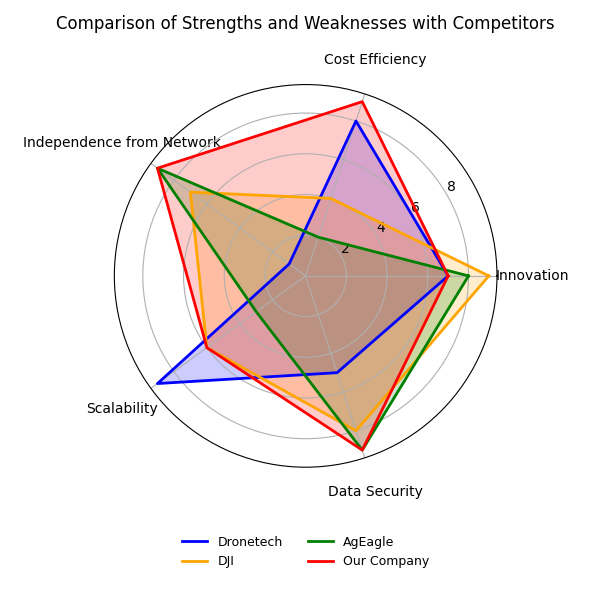
\includegraphics[width=400pt]{figures/competitors.png} 
	\caption{Comparison of Strengths and Weaknesses with Competitors}
	\source{Own illustration created with Matplotlib in Python}
	\label{fig:strengths_weaknesses} 
\end{figure}

Our ground-based \acrshort{3d} drone tracking system offers an affordable and independent solution for Austria's agricultural sector. By using calibrated ground stations with advanced image processing, we eliminate the need for expensive onboard positioning and obstacle avoidance systems. This allows to deploy simpler drones, reducing costs, maintenance complexities, and payload restrictions. As a result, small to medium enterprises can access modern drone technology, overcoming challenges like network coverage limitations and high equipment costs, making it a practical tool for improving farming operations without substantial investment.

Our approach provides several key benefits:

\begin{itemize} 
	\item \textbf{Enhanced Efficiency and Cost Savings:} Without heavy onboard sensors, drones are lighter and consume less energy, thus increasing flight times and coverage area. They can carry more payloads like seeds, fertilizers, or pesticides, enhancing operational efficiency. Reduced complexity lowers maintenance and failure risk, leading to cost savings and making precision agriculture accessible to farmers with limited budgets.
	
	\item \textbf{Secure, Independent Communication:} Our local communication system operates independently of network infrastructure, ensuring reliability in areas with connectivity issues. Unlike competitors relying on 5G, our system enhances reliability, data security, and privacy by processing tracking data locally.
	
	\item \textbf{Scalability and Flexibility:} Our ground stations can track multiple drones simultaneously without adding complexity or weight to drones. This enables scalable operations, allowing farmers to expand fleets without significant additional investment.

\end{itemize}

\section{Conclusion}

The market analysis reveals a significant opportunity for our ground-based \acrshort{3d} drone tracking system in the agricultural sector. As drone adoption in agriculture accelerates, our solution addresses key challenges like high costs, dependence on network infrastructure, and the complexity of onboard systems by eliminating the need for expensive onboard positioning, and obstacle avoidance equipment. By enabling the use of simpler, more affordable drones with increased payload capacity and simplified maintenance, we offer a unique value proposition that differentiates us from competitors relying on complex onboard technologies. Our system aligns with the needs of small to medium agricultural enterprises seeking efficient and sustainable technologies without the barriers of high initial investment and technical complexity. Further research and engagement with industry stakeholders will refine our understanding of target customers and support a successful market entry, positioning us as a competitive player in the agricultural drone market focused on accessibility and practicality.


% 
\chapter{Latex-Beispiele}
\label{chap:bsp}

\section{Aulistungen}

\begin{itemize}
	\item \textit{Kursiv} Text 1
	\item \textbf{Fett}  
	\item \texttt{TT} 
	\end{itemize}
	
	Dasselbe durchnumeriert:
	
	\begin{enumerate}
		\item \textit{Kursiv} Text 1
		\item \textbf{Fett}  
		\item \texttt{TT} 
	\end{enumerate}


\section{Tabellen}

Eine Tabelle mit Testdaten:


\begin{table}[H]
	\begin{center}
		\begin{tabular}{lrrrrr}\hline\hline
			\multicolumn{1}{l}{\textbf{position}}&
			\multicolumn{1}{c}{\textbf{mean}}&
			\multicolumn{1}{c}{\textbf{median}}&
			\multicolumn{1}{c}{\textbf{sd}}&
			\multicolumn{1}{c}{\textbf{min}}&
			\multicolumn{1}{c}{\textbf{max}}
			\\ \hline
			\textbf{6}&$6.89$&$5.61$&$ 7.29$&$0.31$&$160.12$\\
			\textbf{9}&$5.35$&$4.39$&$ 4.94$&$0.18$&$ 76.40$\\
			\textbf{12}&$8.70$&$6.96$&$10.72$&$0.15$&$239.88$\\
			\textbf{13}&$9.01$&$7.54$&$ 7.60$&$0.15$&$138.86$\\
			\textbf{15}&$8.18$&$6.99$&$ 6.86$&$0.16$&$117.26$\\
			\textbf{16}&$5.26$&$4.42$&$ 4.99$&$0.08$&$110.21$\\
			\textbf{17}&$5.87$&$4.79$&$ 6.13$&$0.15$&$ 98.88$\\
			\textbf{36}&$8.21$&$6.72$&$ 7.58$&$1.36$&$122.35$\\
			\textbf{42}&$6.77$&$5.93$&$ 6.98$&$1.72$&$123.72$\\
			\textbf{43}&$6.27$&$5.53$&$ 3.21$&$0.57$&$ 35.69$\\
			\hline
		\end{tabular}
	\end{center}
	\caption{Eine Tabelle mit Testdaten} 
	\label{tabelle:test}
\end{table}

Sprachen wie z.B. \textbf{R} können Latex-Tabellen exportieren, sie müssen also nicht immer so aufwändig formatiert werden.			


\section{Abbildungen}

 \begin{figure}[H]
 	%\centering
 	\hspace*{-1.5cm}
 	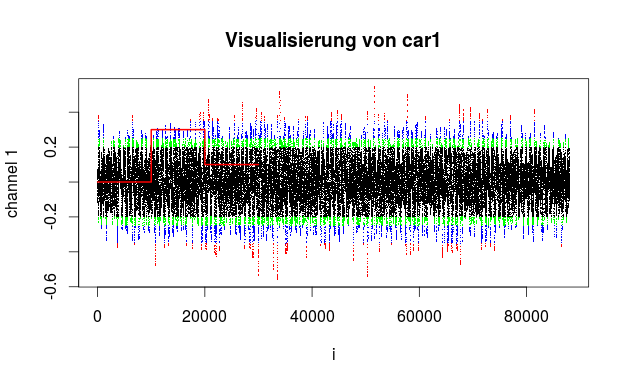
\includegraphics[width=512pt,height=280pt]{figures/bsp.png}
 	\caption{Ein Beispiel für ein Bild}
 	\label{bild:beispiel}
 \end{figure}
 
 
\section{Quellcode}

Quellcode wird automatisch (mit der Möglichkeit die Sprache anzugeben) formatiert und in das Listings-Verzeichnis gegeben:

\subsection{Java-Code}

\begin{lstlisting}[style=Java, caption={Java-Beispiel}, captionpos=b]
int i = 1;
float f = 2;
System.out.printf("Int-Z %d Float-Z: 52f",i ,f );
\end{lstlisting} 


\subsection{Python-Code}
 
\begin{lstlisting}[style=Python, caption={Python-Beispiel}, captionpos=b]
#Hier ein kleines Beispiel in Python
lower = 0
upper = 10
for i in range(lower,upper):
print(i)
\end{lstlisting} 


\subsection{Lesen von Dateien}
 
Es kann auch direkt von Dateien gelesen werden:

\lstinputlisting[style=Java, label={java_bsp}, caption={Java-Beispiel von Datei}, captionpos=b]{sourcecode/First.java}
 
\section{Referenzen}
			
Beispiele für die Verwendung von Referenzen: 

\begin{itemize}
	\item Wie in Tabelle ~\ref{tabelle:test} ersichtlich... 
	\item Wir sind im Kapitel ~\ref{chap:bsp}
	\item In Zeile 2 im Listing ~\ref{java_bsp} 
\end{itemize}


\section{Zitate}


Hier das Zitat eines Buches: \cite{couper2001} Wird alles automatisch mit  bibtex erledigt. % Einfach auskommentieren für die tatsächliche Arbeit

\appendix                       %% closes main document, appendix follows until end; only available in book-classes

\addpart*{Appendix}             %% adding Appendix to tableofcontents

\printglossary

\listoftables
\listoffigures
\lstlistoflistings
\nocite{*} %Es werden auf nicht referenzierte Literaturstellen aufgelistet
\bibliography{references}

\end{document}
